\documentclass[a4paper,11pt]{book}
%\documentclass[a4paper,twoside,11pt,titlepage]{book}
\usepackage{listings}
\usepackage[utf8]{inputenc}
\usepackage[spanish]{babel}
\usepackage{float}
\usepackage{tabularx}
\renewcommand\tabularxcolumn[1]{m{#1}}
\usepackage{amsmath}

\newcommand{\tabitem}{~~\llap{\textbullet}~~}

% GANTT
\usepackage[spanish]{translator}

\usepackage{pgfgantt}
\def\pgfcalendarweekdayletter#1{%
\ifcase#1L\or M\or X\or J\or V\or S\or D\fi%
}

% FIN GANTT

% \usepackage{xcolor}      % PARA PONER COLOR AL TEXTO
\usepackage{xspace}

\setcounter{secnumdepth}{3}
\setcounter{tocdepth}{3}
% \usepackage[style=list, number=none]{glossary} %
%\usepackage{titlesec}
%\usepackage{pailatino}

\decimalpoint
\usepackage{dcolumn}
\newcolumntype{.}{D{.}{\esperiod}{-1}}
\makeatletter
\addto\shorthandsspanish{\let\esperiod\es@period@code}
\makeatother


%\usepackage[chapter]{algorithm}
\RequirePackage{verbatim}
%\RequirePackage[Glenn]{fncychap}
\usepackage{fancyhdr}
\usepackage{graphicx}
\usepackage{afterpage}

\usepackage{longtable}

\usepackage[pdfborder={000}]{hyperref} %referencia
\usepackage{xurl}

% ********************************************************************
% Re-usable information
% ********************************************************************
\newcommand{\myTitle}{Título del proyecto\xspace}
\newcommand{\myDegree}{Grado en Ingeniería Informática\xspace}
\newcommand{\myName}{Andrés Merlo Trujillo\xspace}
\newcommand{\myProf}{Luis López Escudero\xspace}
%\newcommand{\myOtherProf}{Nombre Apllido1 Apellido2 (tutor2)\xspace}
%\newcommand{\mySupervisor}{Put name here\xspace}  NO USADO
\newcommand{\myFaculty}{Escuela Técnica Superior de Ingenierías Informática y de
Telecomunicación\xspace}
\newcommand{\myFacultyShort}{E.T.S. de Ingenierías Informática y de
Telecomunicación\xspace}
\newcommand{\myDepartment}{Departamento de Lenguaje y Sistemas Informáticos\xspace}
\newcommand{\myUni}{\protect{Universidad de Granada}\xspace}
\newcommand{\myLocation}{Granada\xspace}
\newcommand{\myTime}{\today\xspace}
\newcommand{\myVersion}{Version 0.1\xspace}
\newcommand{\sprintNro}{3\xspace}
\newcommand{\sprintLength}{2 semanas\xspace}
\newcommand{\actualSprintLength}{10 días\xspace}
\newcommand{\projectph}{20 PH\xspace}

\hypersetup{
pdfauthor = {\myName (andresmerlo@correo.ugr.es)},
pdftitle = {\myTitle},
pdfsubject = {},
pdfkeywords = {Unreal, Simulación, IA },
pdfcreator = {LaTeX con el paquete ....},
pdfproducer = {pdflatex}
}

%\hyphenation{}


%\usepackage{doxygen/doxygen}
%\usepackage{pdfpages}
\usepackage{url}
\usepackage{colortbl,longtable}
\usepackage[stable]{footmisc}
%\usepackage{index}

%\makeindex
%\usepackage[style=long, cols=2,border=plain,toc=true,number=none]{glossary}
% \makeglossary

% Definición de comandos que me son tiles:
%\renewcommand{\indexname}{Índice alfabético}
%\renewcommand{\glossaryname}{Glosario}

\pagestyle{fancy}
\fancyhf{}
\fancyhead[LO]{\leftmark}
\fancyhead[RE]{\rightmark}
\fancyhead[RO,LE]{\textbf{\thepage}}
\renewcommand{\chaptermark}[1]{\markboth{\textbf{#1}}{}}
\renewcommand{\sectionmark}[1]{\markright{\textbf{\thesection. #1}}}

\setlength{\headheight}{1.5\headheight}

\newcommand{\HRule}{\rule{\linewidth}{0.5mm}}
%Definimos los tipos teorema, ejemplo y definición podremos usar estos tipos
%simplemente poniendo \begin{teorema} \end{teorema} ...
\newtheorem{teorema}{Teorema}[chapter]
\newtheorem{ejemplo}{Ejemplo}[chapter]
\newtheorem{definicion}{Definición}[chapter]

\definecolor{gray97}{gray}{.97}
\definecolor{gray75}{gray}{.75}
\definecolor{gray45}{gray}{.45}
\definecolor{gray30}{gray}{.94}

\lstset{ frame=Ltb,
     framerule=0.5pt,
     aboveskip=0.5cm,
     framextopmargin=3pt,
     framexbottommargin=3pt,
     framexleftmargin=0.1cm,
     framesep=0pt,
     rulesep=.4pt,
     backgroundcolor=\color{gray97},
     rulesepcolor=\color{black},
     %
     stringstyle=\ttfamily,
     showstringspaces = false,
     basicstyle=\scriptsize\ttfamily,
     commentstyle=\color{gray45},
     keywordstyle=\bfseries,
     %
     numbers=left,
     numbersep=6pt,
     numberstyle=\tiny,
     numberfirstline = false,
     breaklines=true,
   }
 
% minimizar fragmentado de listados
\lstnewenvironment{listing}[1][]
   {\lstset{#1}\pagebreak[0]}{\pagebreak[0]}

\lstdefinestyle{CodigoC}
   {
	basicstyle=\scriptsize,
	frame=single,
	language=C,
	numbers=left
   }
\lstdefinestyle{CodigoC++}
   {
	basicstyle=\small,
	frame=single,
	backgroundcolor=\color{gray30},
	language=C++,
	numbers=left
   }

 
\lstdefinestyle{Consola}
   {basicstyle=\scriptsize\bf\ttfamily,
    backgroundcolor=\color{gray30},
    frame=single,
    numbers=none
   }


\newcommand{\bigrule}{\titlerule[0.5mm]}


%Para conseguir que en las páginas en blanco no ponga cabecerass
\makeatletter
\def\clearpage{%
  \ifvmode
    \ifnum \@dbltopnum =\m@ne
      \ifdim \pagetotal <\topskip
        \hbox{}
      \fi
    \fi
  \fi
  \newpage
  \thispagestyle{empty}
  \write\m@ne{}
  \vbox{}
  \penalty -\@Mi
}
\makeatother

\usepackage{pdfpages}
\begin{document}
\begin{titlepage}
 
 
\newlength{\centeroffset}
\setlength{\centeroffset}{-0.5\oddsidemargin}
\addtolength{\centeroffset}{0.5\evensidemargin}
\thispagestyle{empty}

\noindent\hspace*{\centeroffset}\begin{minipage}{\textwidth}

\centering

\includegraphics[width=0.9\textwidth]{imagenes/logo_ugr.jpg}\\[1.4cm]

\textsc{ \Large TRABAJO FIN DE GRADO\\[0.2cm]}
\textsc{ INGENIERÍA EN ...}\\[1cm]
% Upper part of the page
% 
% Title
{\Huge\bfseries Titulo del Proyecto\\
}
\noindent\rule[-1ex]{\textwidth}{3pt}\\[3.5ex]
{\large\bfseries Subtitulo del Proyecto}
\end{minipage}

\vspace{2.5cm}
\noindent\hspace*{\centeroffset}\begin{minipage}{\textwidth}
\centering

\textbf{Autor}\\ {Nombre Apellido1 Apellido2 (alumno)}\\[2.5ex]
\textbf{Directores}\\
{Nombre Apellido1 Apellido2 (tutor1)\\
Nombre Apellido1 Apellido2 (tutor2)}\\[2cm]

\includegraphics[width=0.3\textwidth]{imagenes/etsiit_logo.png}\\[0.1cm]
\textsc{Escuela Técnica Superior de Ingenierías Informática y de Telecomunicación}\\
\textsc{---}\\
Granada, mes de 201
\end{minipage}
%\addtolength{\textwidth}{\centeroffset}
%\vspace{\stretch{2}}
\end{titlepage}



\chapter*{}
%\thispagestyle{empty}
%\cleardoublepage

%\thispagestyle{empty}

\begin{titlepage}
 
 
\setlength{\centeroffset}{-0.5\oddsidemargin}
\addtolength{\centeroffset}{0.5\evensidemargin}
\thispagestyle{empty}

\noindent\hspace*{\centeroffset}\begin{minipage}{\textwidth}

\centering
%
\includegraphics[width=0.9\textwidth]{imagenes/logo_ugr.jpg}\\[1.4cm]

%\textsc{ \Large PROYECTO FIN DE CARRERA\\[0.2cm]}
%\textsc{ INGENIERÍA EN INFORMÁTICA}\\[1cm]
% Upper part of the page
% 

 \vspace{3.3cm}

%si el proyecto tiene logo poner aquí

\includegraphics{imagenes/logo.png} 
 \vspace{0.5cm}

% Title

{\Huge\bfseries Título del proyecto\\
}
\noindent\rule[-1ex]{\textwidth}{3pt}\\[3.5ex]
{\large\bfseries Subtítulo del proyecto.\\[4cm]}
\end{minipage}

\vspace{2.5cm}
\noindent\hspace*{\centeroffset}\begin{minipage}{\textwidth}
\centering

\textbf{Autor}\\ {Nombre Apellido1 Apellido2 (alumno)}\\[2.5ex]
\textbf{Directores}\\
{Nombre Apellido1 Apellido2 (tutor1)\\
Nombre Apellido1 Apellido2 (tutor2)}\\[2cm]
%
\includegraphics[width=0.15\textwidth]{imagenes/tstc.png}\\[0.1cm]
%\textsc{Departamento de Teoría de la Señal, Telemática y Comunicaciones}\\
%\textsc{---}\\
%Granada, mes de 201
\end{minipage}
%\addtolength{\textwidth}{\centeroffset}
\vspace{\stretch{2}}

 
\end{titlepage}






\cleardoublepage
\thispagestyle{empty}

\begin{center}
{\large\bfseries \myTitle}\\
\end{center}
\begin{center}
Andrés Merlo Trujillo\\
\end{center}

%\vspace{0.7cm}
\noindent{\textbf{Palabras clave}: Unreal, Simulación, IA }\\

\vspace{0.7cm}
\noindent{\textbf{Resumen}}\\

Se pretende desarrollar una aplicación gráfica utilizando el motor gráfico \textit{Unreal Engine}, cuyo objetivo es de poder simular carreras de coches. Esta simulación dotará a los pilotos virtuales de la capacidad de tomar decisiones realistas y de cometer errores, basándose en las condiciones de cada piloto durante la carrera, que pueden variar dependiendo de las condiciones externas o ser modificadas por el usuario en tiempo real. Además, se podrán configurar ajustes adicionales antes de comenzar la carrera, con el objetivo de hacer la simulación lo más personalizable posible.

\cleardoublepage


\thispagestyle{empty}


\begin{center}
{\large\bfseries Car racing simulator in Unreal Engine}\\
\end{center}
\begin{center}
Andrés Merlo Trujillo\\
\end{center}

%\vspace{0.7cm}
\noindent{\textbf{Keywords}: Unreal, Simulation, AI }\\

\vspace{0.7cm}
\noindent{\textbf{Abstract}}\\

The aim is to develop a graphics application using the graphics engine \textit{Unreal Engine}, whose objective is to be able to simulate car races. This simulation will provide virtual pilots with the ability to make realistic decisions and make mistakes, based on the conditions of each pilot during the race, which can vary depending on external conditions or be modified by the user in real time. Furthermore, additional settings can be configured before starting the race, with the aim of making the simulation as customizable as possible.

\chapter*{}
\thispagestyle{empty}

\noindent\rule[-1ex]{\textwidth}{2pt}\\[4.5ex]

Yo, \textbf{Andrés Merlo Trujillo}, alumno de la titulación Ingeniería Informática de la \textbf{Escuela Técnica Superior
de Ingenierías Informática y de Telecomunicación de la Universidad de Granada}, con DNI 77147239H, autorizo la
ubicación de la siguiente copia de mi Trabajo Fin de Grado en la biblioteca del centro para que pueda ser
consultada por las personas que lo deseen.

\vspace{6cm}

\noindent Fdo: Andrés Merlo Trujillo

\vspace{2cm}

\begin{flushright}
Granada a 11 de julio de 2023.
\end{flushright}


\chapter*{}
\thispagestyle{empty}

\noindent\rule[-1ex]{\textwidth}{2pt}\\[4.5ex]

D. \textbf{Luis López Escudero}, Profesor del Área del Departamento de Lenguajes y Sistemas Informáticos de la Universidad de Granada.

\vspace{0.5cm}

D. \textbf{Germán Arroyo Moreno}, Profesor del Área del Departamento de Lenguajes y Sistemas Informáticos de la Universidad de Granada.


\vspace{0.5cm}

\textbf{Informan:}

\vspace{0.5cm}

Que el presente trabajo, titulado \textit{\textbf{\myTitle}},
ha sido realizado bajo su supervisión por \textbf{Andrés Merlo Trujillo}, y autorizamos la defensa de dicho trabajo ante el tribunal
que corresponda.

\vspace{0.5cm}

Y para que conste, expiden y firman el presente informe en Granada a 11 de julio de 2023.

\vspace{1cm}

\textbf{Los directores:}

\vspace{5cm}

\noindent \textbf{Luis López Escudero \ \ \ \ \ Germán Arroyo Moreno}

\chapter*{Agradecimientos}
\thispagestyle{empty}

       \vspace{1cm}


A mi familia y a los tutores por brindarme su apoyo durante todo el desarrollo del proyecto.



%\frontmatter
\tableofcontents
\newpage
%\listoffigures
%\listoftables
%
%\mainmatter
% \setlength{\parskip}{5pt}

\chapter{Introducción}
\section{Introducción y Motivación}
%PALABRAS REPETIDAS, REVISAR
%gran cantidad
%no se repite, pero "cosas" queda muy feo

El mundo del motor es un deporte con una amplia base de seguidores y en el que se invierte una gran cantidad de dinero en simuladores de todo tipo para poder tener una ventaja competitiva. Estos simuladores permiten a los equipos de carreras realizar una extensa variedad de actividades: entrenar a los pilotos antes y durante la temporada, modificar parámetros para lograr el máximo rendimiento del vehículo o simular carreras para analizar cuál será la estrategia más adecuada para alcanzar la victoria.

\bigskip

El proyecto se centrará en la simulación de gestión de carreras, sector donde existen pocas opciones para el público general y que es cada vez más demandado para aprender la manera en que las distintas estrategias pueden afectar al desenlace de una carrera y como diferentes situaciones influyen en la capacidad de los pilotos. Estos factores pueden afectar a la tasa de errores producidos durante la carrera.

% \bigskip

% Se añadirán ciertas características procedentes de videojuegos con elementos de simulación a la aplicación gráfica, como la posibilidad de elegir entre varios tipos de vehículos y algunas de las aptitudes de los pilotos, ambas procedentes de \textit{Gran Turismo B-Spec}

\bigskip


La motivación detrás de realizar este programa es profundizar en los conocimientos previamente adquiridos en otras asignaturas del manejo de \textit{Unreal Engine} y en el aprendizaje de su API, enfocándolo al ámbito de las carreras y de los vehículos autónomos, área que me resulta muy interesante. Asimismo, se busca profundizar en el estudio de los distintos algoritmos de navegación para los vehículos del simulador, intentando escoger el que mejor se adapte a las necesidades del proyecto y que ofrezca buenos resultados.

\newpage

\section{Objetivos}

En este proyecto se pretende desarrollar un simulador de gestión de carreras multidisciplinar y personalizable, cuyos pilotos tendrán un conjunto de capacidades que serán modificadas por las condiciones de la carrera o por el usuario en tiempo real, haciendo que el piloto pueda cometer más errores o menos si su estado mejora. También existirá la opción de poder modificar la velocidad de simulación, con el objetivo de obtener los resultados de manera más rápida.

\bigskip

Además, la aplicación permitirá modificar diversos parámetros antes de la carrera, con el propósito de personalizar la simulación lo máximo posible. Cabe destacar que estos parámetros no podrán ser cambiados de nuevo, debido a que no tendría demasiado sentido y podrían hacer que los resultados finales no fueran del todo precisos.


\bigskip


Siendo más específicos, los objetivos mínimos relativos a alteraciones antes de ejecutar la simulación son:

\begin{itemize}
   \item Cambio de número de pilotos.
   \item Cambio de número de vueltas.
   \item Cambio de las características de los pilotos.
   \item Cambio del tipo de vehículo.
\end{itemize}

\bigskip

En cuanto a cambios durante la carrera, debe cumplir estos objetivos:

\begin{itemize}
   % \item Seleccionar piloto de la lista de pilotos.
   \item Obtener las condiciones actuales de cada piloto.
   \item Modificar las condiciones actuales de un piloto concreto.
   \item Cambiar la velocidad de simulación.
   \item Cambiar la perspectiva de la cámara.
\end{itemize}

Conviene resaltar que todos estos objetivos y algunos opcionales serán explicados en detalle en apartados siguientes.

\section{Estado del arte}
Como ya se ha descrito anteriormente, este proyecto hará uso de \textit{Unreal Engine} como motor gráfico y \textit{framework} para la realización del simulador especificado. En cuanto a la forma en la que los pilotos se moverán por el circuito, he decidido usar el algoritmo de navegación \finalAlg.

\bigskip

A continuación, voy a explicar las distintas opciones que hay disponibles en motores gráficos y en algoritmos de navegación y explicar el motivo de la elección realizada. Separaré esto en dos subsecciones.

\subsection{Motor gráfico}
En el mercado hay gran variedad de motores gráficos de videojuegos, los más conocidos son los siguientes:

\subsubsection{Unreal Engine}

\begin{figure}[H]
   \centering
   
\includegraphics[width=0.3\textwidth]{imagenes/UE_LOGO.png}
   \caption{Logotipo de \textit{Unreal Engine}\cite{unreal-logo}.}
   % \vspace{10pt}
   % \footnotesize{Fuente: \url{https://es.wikipedia.org/wiki/Unreal_Engine}}
\end{figure}

Unreal Engine \cite{unreal} es una plataforma de desarrollo que permite, entre otras cosas: el desarrollo de videojuegos, creación de contenido para programas y películas, simulación, etc. Posee un soporte para un gran número de plataformas, tanto consolas como móviles.

\bigskip

Unreal incluye \textit{Blueprint Visual Scripting}, el cual es un sistema de \textit{scripting} visual que hace uso de nodos para programar las distintas partes del sistema. Permite programar de manera visual sin la necesidad de conocer la \textit{API} de C++.

\bigskip

Además, a partir de la versión 5.0, Unreal incluye diversas tecnologías como: 

\begin{itemize}
   \item TSR \textit{(Temporal Super Resolution)}, que mejora el rendimiento haciendo que el juego se renderice internamente a una resolución menor y luego sea reescalado al tamaño deseado.
   \item Nanite, que permite tener objetos con una gran cantidad de polígonos en la pantalla, 
   \item Lumen, que genera una iluminación más realista.
\end{itemize}

Estas tecnologías permiten obtener un resultado gráfico muy convincente, partiendo de un modelo creado por profesionales. Asimismo, la inclusión de \textit{TSR} posibilita escalar la aplicación a resoluciones mayores de lo que el hardware es capaz de ejecutar.

\bigskip

Unreal también incluye una tienda con abundantes recursos, permitiendo simplificar mucho el desarrollo de videojuegos.

\bigskip

Sin embargo, no tiene una licencia de código abierto, pero su código fuente es accesible a través de un repositorio de GitHub.

\subsubsection{Unity}

\begin{figure}[H]
   \centering
   
\includegraphics[width=0.4\textwidth]{imagenes/UNITY_LOGO.png}
   \caption{Logotipo de \textit{Unity}\cite{unity}.}
   % \vspace{10pt}
   % \footnotesize{Fuente: \url{https://es.wikipedia.org/wiki/Unity_(motor_de_videojuego)}}
\end{figure}

Unity \cite{unity} es una plataforma de desarrollo que permite: desarrollar videojuegos, visualizar construcciones en el ámbito de la arquitectura, para uso en la industria automotriz y para la creación de películas y series.

\bigskip

Entre sus características se encuentra:

\begin{itemize}
   \item Uso de C\# como lenguaje de programación.
   \item Motor de físicas 2D separado del de físicas en 3D.
   \item Posee un \textit{Scriptable Rendering Pipeline} altamente personalizable, permitiendo mediante el uso de scripts escritos en C\# personalizar sombras, iluminación, oclusión ambiental, entre otras.
   \item Soporte para un gran número de plataformas, incluyendo consolas y móviles, aparte de Windows, macOS y Linux.
   \item Incluye un lenguaje de programación visual, similar a \textit{Unreal} que permite programar sin necesitar conocer la \textit{API}.
\end{itemize}
   
Además, Unity tiene varias versiones del programa, incluyendo uno gratuito y los demás de pago, con prioridad de asistencia y un mayor abanico de herramientas.

\subsubsection{Godot}

\begin{figure}[H]
   \centering
   
\includegraphics[width=0.4\textwidth]{imagenes/GODOT_LOGO.png}
   \caption{Logotipo de \textit{Godot}\cite{godot-logo}.}
   % \vspace{10pt}
   % \footnotesize{Fuente: \url{https://es.wikipedia.org/wiki/Godot}}
\end{figure}

Godot \cite{godot} es un motor gráfico gratuito y multiplataforma de código abierto que permite crear videojuegos en 2D y 3D. 

\bigskip

Entre las características más notables se encuentran las siguientes:

\begin{itemize}
   \item Motor gráfico 2D dedicado. 
   \item Programación usando GDScript, C\# o C++ de manera oficial. No obstante, se puede programar usando otro lenguaje como Rust, Python o JavaScript. 
   \item Soporte para un gran número de plataformas, incluyendo móviles y consolas.
   \item Incluye un motor de físicas (solo para el motor gráfico 3D), aunque es algo más simple que el de sus competidores.
\end{itemize}

\bigskip 

A partir de la versión 4, Godot ha dejado de incluir el lenguaje visual, debido a su falta de uso, por lo que solo es posible utilizar lenguajes de programación convencionales \cite{godot-no-visual}.

\bigskip

Además, Godot tiene una biblioteca con una gran cantidad de recursos para utilizar durante el desarrollo de un videojuego.


\subsubsection{Elección final}

Al final, he decidido utilizar Unreal Engine debido a que la versión gratuita incluye toda la funcionalidad, es el más potente en cuanto a programación visual y es con el que más familiarizado estoy de todas las opciones citadas anteriormente.

\subsection{Algoritmo de navegación}
En cuanto a algoritmos de navegación para los vehículos, los más destacados son:

\begin{itemize}
   \item \textbf{Aprendizaje por refuerzo:} Es una técnica de aprendizaje automático en la que el agente aprende a tomar decisiones en un entorno mediante la interacción a través de acciones
   y recibiendo una recompensa en caso de acercarse al objetivo deseado o de hacerlo bien. 
   
   Es importante obtener un equilibrio entre exploración y explotación, de forma que sea capaz de actuar ante situaciones desconocidas correctamente. En caso de estar desequilibrado, puede darse la situación en el que se produzca un máximo local y no sea capaz de descubrir la mejor estrategia.

   
   Para evitar esto, se suelen utilizar métodos de equilibrio. Uno de ellos es el denominado \textit{epsilon-greedy}, que permite controlar la cantidad de exploración mediante un parámetro \textit{epsilon}, que determina la aleatoriedad en la selección de acciones \cite{10.1007/978-3-642-24455-1_33}, permitiendo elegir en función de dicho parámetro una acción aleatoria o la mejor hasta el momento.

   Una desventaja que tiene es la necesidad de entrenar el modelo, lo cual puede ser un proceso largo y complicado, pero con el suficiente tiempo y con un conjunto de recompensas y castigos bien realizado, es una excelente técnica para resolver este tipo de problema.

   El algoritmo \textit{Q-Learning} es uno de los más utilizados para espacios discretos. Consiste en una función Q, la cual posibilita al agente estimar el valor esperado de una acción dado un estado. Dicha función se implementa mediante una tabla denominada \textit{Q-Values}, la cual almacena el valor esperado de las recompensas para cada estado y acción posible. Para evitar problemas de equilibrio, se utilizan métodos como el \textit{epsilon-greedy}, ampliamente utilizado y que ofrece buenos resultados.

   No obstante, si el entorno de aprendizaje es continuo, una tabla de \textit{Q-Values} no es adecuada debido a la gran cantidad de posibles valores y el alto costo computacional en procesamiento y memoria. En su lugar, se puede sustituir la tabla por una red neuronal, como el algoritmo \textit{Deep Q-Network} (DQN), para trabajar en este tipo de espacios \cite{coulom:tel-00003985}.

   Para este proyecto, se podría implementar DQN. La red neuronal tendría como entrada varios sensores de colisión y de límites de pista, y como salida el nivel de aceleración, frenado y giro del volante.

   \item \textbf{Mediante reglas:} Conjunto de acciones que se aplican cuando se cumple una determinada condición y suelen estar ordenadas por prioridad. Pueden ser representadas mediante un árbol, donde cada acción se encuentra en una hoja y las preguntas o condiciones que las activan son las ramas (aristas). La prioridad de las acciones se establece según su posición en el árbol, siendo las más importantes las de niveles superiores.
   
   Esto tiene la ventaja de ser más sencillo de implementar que el de aprendizaje por refuerzo, pero suele tener peores resultados, al poder darse el caso de no haber priorizado bien las reglas o no haber tenido en cuenta algún caso especial.


   Aplicado a este proyecto, se podría diseñar como un conjunto de funciones que manejen cada posible control del vehículo y se ejecuten de manera periódica. De esta forma, dependiendo del entorno y del estado del piloto, se aplicarán distintas salidas para guiar el vehículo por el circuito.

   \item \textbf{Máquina de estados:} Este algoritmo implementa una máquina de estados finitos mediante una estructura de datos, donde cada nodo representa la estrategia seguida y cada arco representa la transición a otro estado. 
   
   Una de las ventajas que tiene es que suele ser más simple describir el comportamiento en agentes más complejos y además, suelen ser más fáciles de modificar que los basados en reglas.

   En este proyecto se podrían implementar estados como: ``Seguir línea'', ``Adelantar'', ``Comienzo de carrera'' y ``Esquivar obstáculo''. Dependiendo del entorno y del estado del piloto, el agente puede pasar a otro estado más adecuado.

   \item \textbf{Algoritmo A* (A Estrella)}: Algoritmo de búsqueda de caminos en grafos que se utiliza para encontrar la ruta óptima. Utiliza una función heurística para guiar la búsqueda hacia la solución más eficiente y es más rápido en tiempo de ejecución que otros algoritmos similares, como el de Dijkstra.
   
   Si se desea aplicar este algoritmo al proyecto, es necesario discretizar el espacio, lo que puede provocar una pérdida de precisión. Además, puede resultar más costoso que otras alternativas anteriormente mencionadas, al poder ser necesario recalcular la ruta.

   No obstante, es un algoritmo de navegación ampliamente utilizado en la industria de los videojuegos, permitiendo realizar modificaciones a la heurística y a la malla de navegación para que se adapte lo máximo posible a las condiciones del proyecto.

   Por tanto, A* podría ser considerado como una opción viable para la navegación por el circuito.

   % No obstante, una ventaja significativa del algoritmo es que se puede incluir el estado del piloto en la función heurística, lo que facilita su integración en el simulador. También se puede aplicar una función de suavizado a la trayectoria resultante para mejorar su precisión. Dado que el proyecto no se centra en la eficiencia computacional, A* podría ser considerado como una opción viable para la navegación por el circuito.
\end{itemize}

% DUDAS
% LAS REFERENCIAS DEBERIAN IR EN LAS REFERENCIAS DEL DOCUMENTO EN GENERAL
% LA CALIDAD DEL DOCUMENTO ES PESIMA
% LOS REQUISITOS DE INFORMACION SON NO FUNCIONALES
% HE REPETIDO DEMASIADAS VECES LO QUE HACE MI SIMULADOR
% EN LA MAYORIA DE LAS SECCIONES HE RELLENADO MAS BIEN POCO
% ME PARECEN POCOS REQUISITOS EN GENERAL, PERO NO SE ME OCURREN MAS

% DUDAS TUTORIA
%no se si poner aqui lo de la pagina web. tipo, que no hay suficientes opciones software para el publico general.


% TODO
% PONER QUE NOS REFERIMOS A SOFTWARE, SISTEMA Y ESO A LO MISMO
\chapter{Especificación de requisitos}

\section{Introducción}

\subsection{Propósito}
%mejorar
El objetivo de esta especificación es definir de manera clara, concisa y precisa las funciones y restricciones que tendrá la aplicación que se desea desarrollar. Al ser un trabajo individual, irá dirigido principalmente a mí, que haré de equipo de desarrollo.

\subsection{Alcance}
%rescribir subsection entera
El proyecto será conocido de ahora en adelante como ``\myTitle''. Por lo tanto, al hacer referencia a ``proyecto'', ``software'', ``simulador'', ``aplicación'' y ``aplicación gráfica'', me referiré a lo mismo.

\bigskip

% repes: carrera
Este sistema se encargará de simular carreras de coches, donde los pilotos tendrán distintas características que variarán dependiendo de las condiciones de la carrera e influirán en su desempeño. El usuario podrá modificar el estado de cada piloto en tiempo real, observando como estos afectan al comportamiento del vehículo.

\bigskip

Además, el software permitirá modificar una serie de ajustes antes de simular la carrera, de acuerdo a las preferencias del usuario. Algunos parámetros son: el número de vehículos, las aptitudes de cada piloto, el tipo de coche y la velocidad máxima. De esta manera, se podrán crear carreras personalizadas de acuerdo a las necesidades del usuario.

\newpage

\subsection{Definiciones, siglas y abreviaturas}

\begin{itemize}
    \item \textbf{Definiciones: }
        \begin{itemize}
            \item \textbf{Usuario: }Persona que utiliza el sistema con el objetivo de obtener los resultados de la carrera personalizada.
            \item \textbf{Simulación: }Se refiere a la ejecución de una carrera en la aplicación.
            \item \textbf{Piloto: }Conductor de un vehículo en la simulación. Será 
            \item \textbf{Aguante mental y físico: }Condiciones que tiene un piloto durante la carrera y que son modificadas durante la simulación, pudiendo afectar a su conducción.
            \item \textbf{Agresividad: }Factor que afectará al piloto durante la carrera, haciendo que si sube cometa más errores.
            \item \textbf{Experiencia: }Parámetro del piloto que no varía durante la carrera y que indica la habilidad que tiene para tomar decisiones.
        \end{itemize}
    \item \textbf{Siglas: }
    \begin{itemize}
        \item \textbf{FPS: }\textit{Frames Per Second}. Son los fotogramas (imágenes) que muestra el sistema cada segundo. Si son lo suficientemente altos, se genera la ilusión de movimiento.
    \end{itemize}
\end{itemize}

% \subsection{Referencias}

% Los siguientes documentos y enlaces se han consultado para crear este capítulo:

% \begin{itemize}
%     \item Ingeniería del Software. Ejercicio en clase, unidad 3: Requerimientos del Software. LSI (UGR). \url{https://lsi2.ugr.es/~mvega/docis/aluwork/colectivo/Ejercicio%20en%20clase%20version%202}
%     \item fusm calidad del software. \url{https://sites.google.com/site/fusmcalidaddelsoftware/proyecto/g-informe-de-especificacion-de-requerimientos/3-requisitos-especificos/3-5-atributos-del-sistema}
% \end{itemize}

\subsection{Visión general}
% rescribir
Este capítulo constará de tres secciones: %Introducción, descripción global, y requisitos específicos. 

\bigskip

En esta primera sección se muestra la introducción y la visión general de la especificación de requisitos.

\bigskip

En la sección 2 se proporcionará una descripción general del sistema a construir, con el fin de conocer las funciones principales, datos requeridos, restricciones y otros aspectos relevantes. 

\bigskip

En la sección 3 se definen detalladamente los requisitos que debe cumplir el sistema en el momento de su desarrollo.

\section{Descripción general}
\subsection{Perspectiva del producto}

\begin{figure}[H]
    \centering
    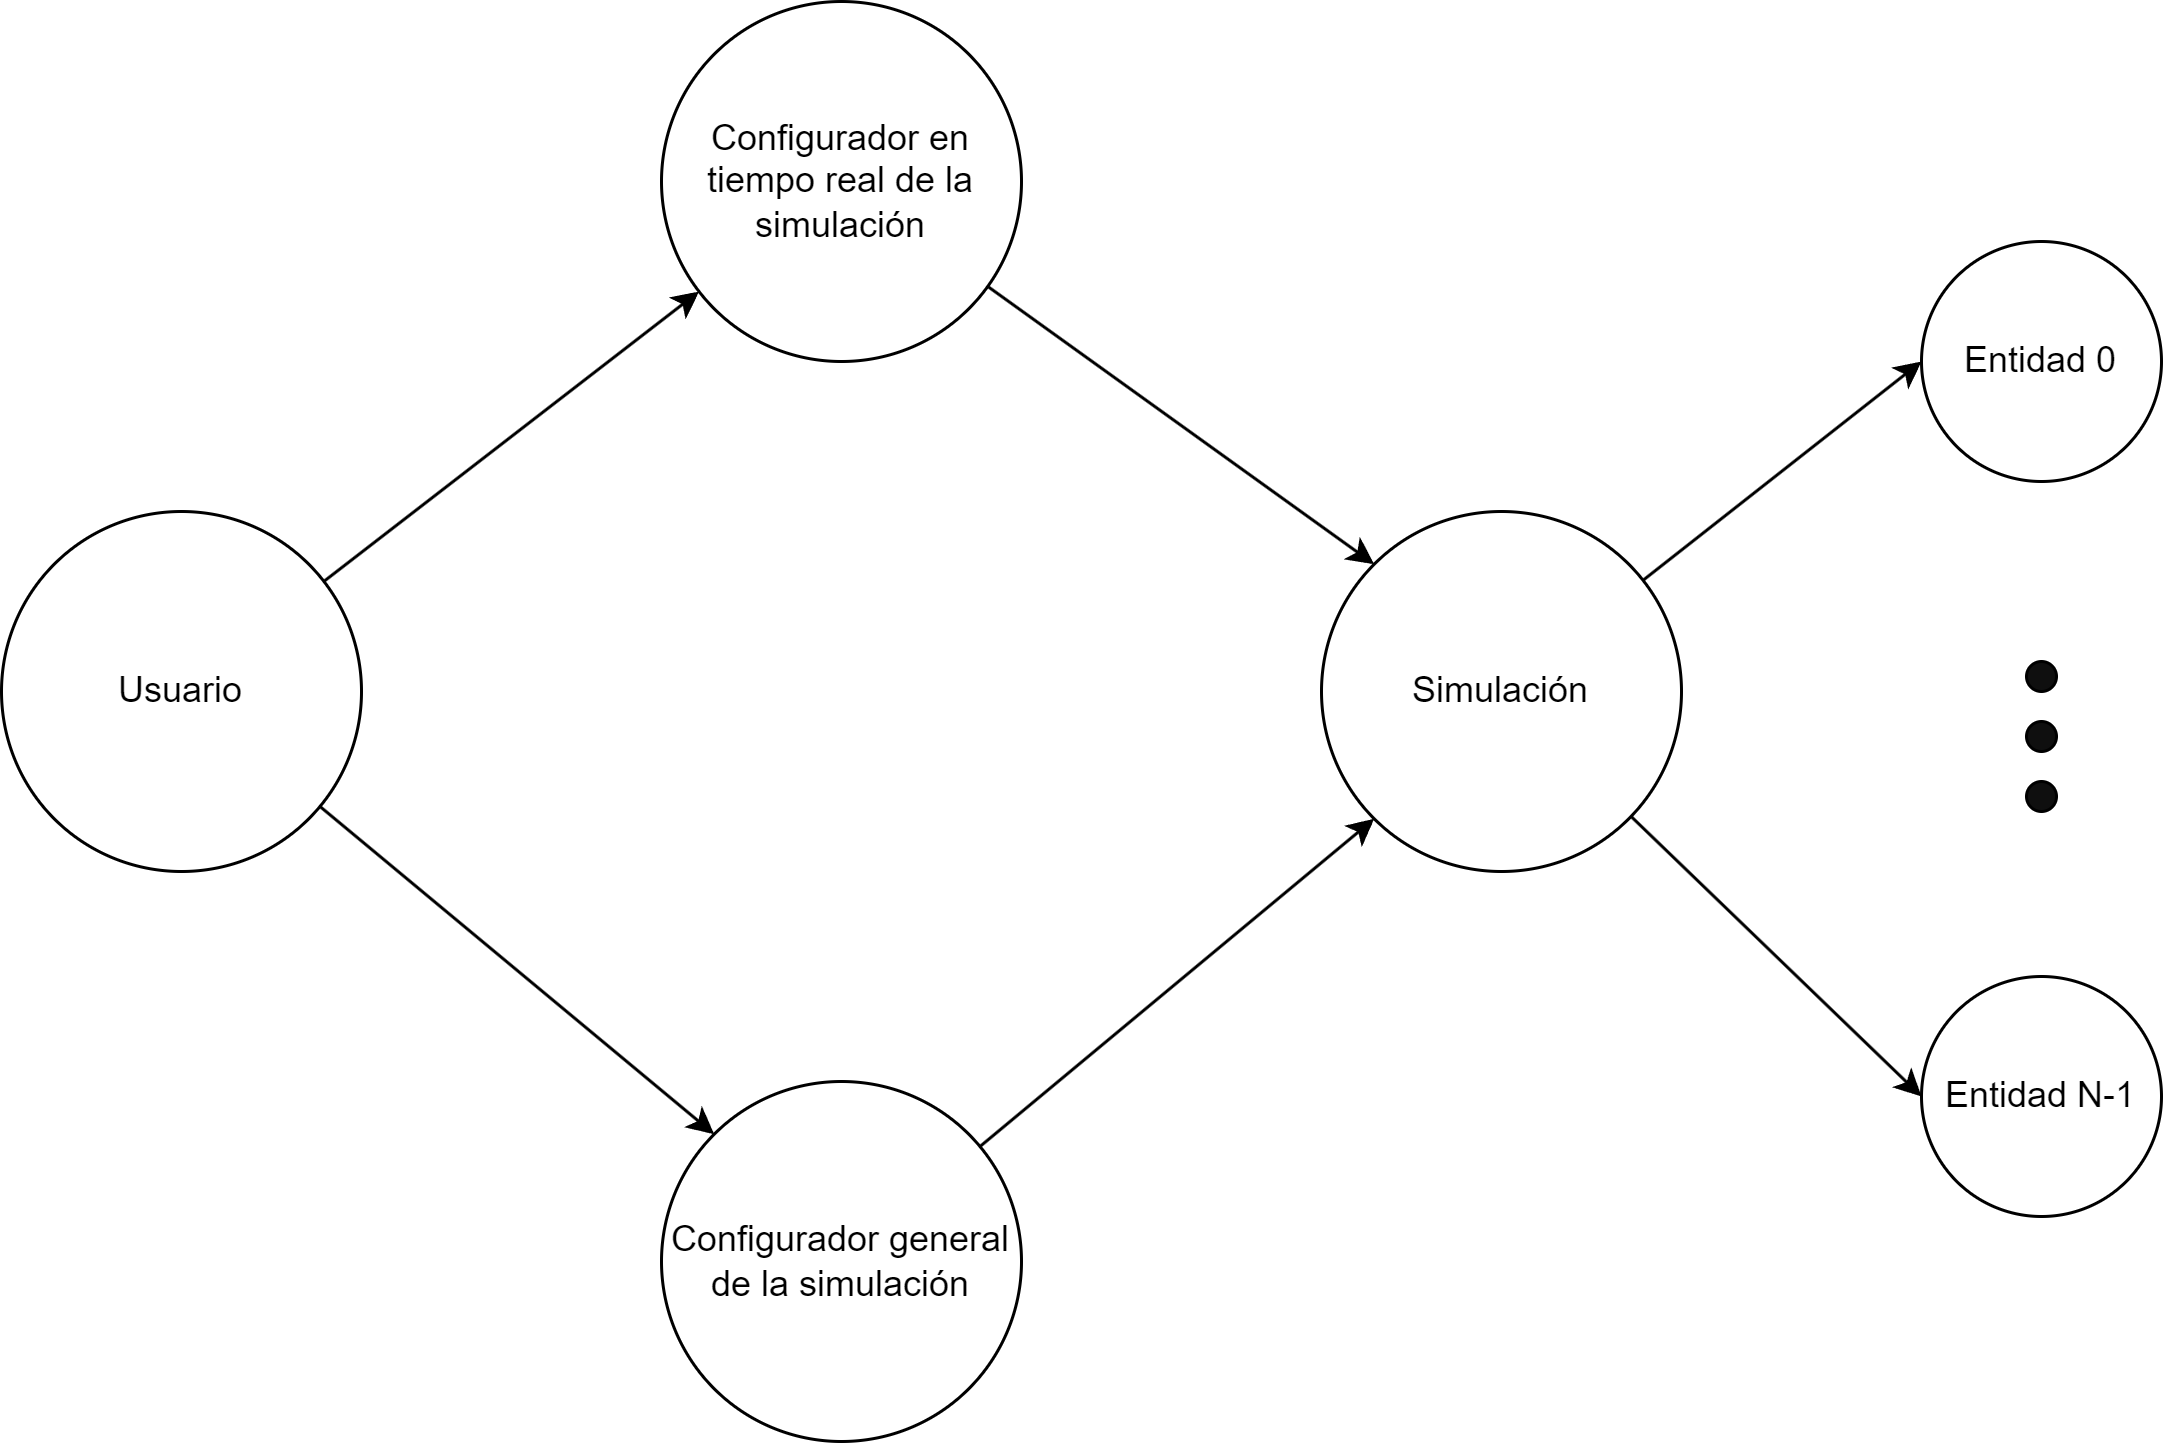
\includegraphics[width=0.8\textwidth]{imagenes/grafo-sistema.drawio.png}
    \caption{Grafo de los distintos componentes del sistema.}
 \end{figure}

El software se diseñará como una aplicación gráfica que permitirá a los usuarios simular carreras de coches, permitiendo configurar parámetros antes de la simulación y durante la carrera. El sistema recopilará información sobre la situación de carrera de cada piloto, y utilizará estos datos para simular el desempeño de cada uno en tiempo real.

\bigskip

Los usuarios interactuarán con el sistema a través de una interfaz gráfica con la que podrán modificar todos los ajustes que estimen convenientes.

\bigskip

Además, será un sistema independiente, al no necesitar interactuar con otros sistemas externos.

\subsection{Funciones del producto}

Las funciones principales de la aplicación son las siguientes:

\begin{itemize}
    \item 
    %Configuración de los parámetros antes de la carrera: 
    % Otorgará la posibilidad de 
    Configurar las distintas opciones antes de la carrera como: número de pilotos, aptitudes de cada uno, tipo de vehículo, velocidad máxima y número de vueltas. 
    
    \item Calcular el estado del piloto según las condiciones actuales de la carrera, de manera que si su estado empeora, cometerá más errores y si mejora, cometerá menos errores, todo en tiempo real.
    
    \item Modificar el estado de los pilotos durante la carrera, con independencia de las condiciones de la misma, pudiendo ver en tiempo real como afecta el cambio producido.
\end{itemize}

Y tendrá otras funciones como:

\begin{itemize}
    \item Pausar la simulación.
    \item Acelerar o reducir la velocidad de simulación.
    \item Cambiar la hora del día.
\end{itemize}

\subsection{Características de los usuarios}

Es recomendable que los usuarios tengan conocimientos básicos de informática, pero no es necesario que sepan como funcionan las carreras, ya que el proceso se encuentra automatizado. 

\subsection{Restricciones}

Las restricciones que tendrá la aplicación son las siguientes:

\begin{itemize}
    \item \textbf{RES1.-} Para el apartado gráfico y la interfaz, se utilizará el motor gráfico \textit{Unreal Engine}.
    \item \textbf{RES2.-} Una vez pausada la simulación, no se podrá modificar su velocidad.
    \item \textbf{RES3.-} El número de pilotos en la carrera no puede ser menor o igual a 1.
    \item \textbf{RES4.-} Las aptitudes de cada piloto antes de la carrera tienen que ser mayores que 0.
    % \item \textbf{RES5.-} La velocidad máxima no podrá ser menor de 150 km/h.
\end{itemize}

\subsection{Suposiciones y dependencias}

% Los requisitos descritos pueden estar sujetos a cambios en función de la evolución del proyecto y la posible adición de nuevas funcionalidades. 

% \bigskip

Este sistema funciona de forma independiente, por lo que no es necesario comunicarse con otros sistemas externos o instalar ningún programa adicional, excepto el propio simulador.

\bigskip

También se asume que el sistema operativo instalado es Windows en sus versiones 10 u 11.

\subsection{Requisitos específicos}

\subsubsection{Requisitos funcionales}

\begin{itemize}
    \item \textbf{RF1.- Modificación de parámetros antes de la carrera:} El sistema debe permitir modificar los parámetros antes de ejecutar la simulación.
    \item \textbf{RF2.- Visualización del estado de los pilotos:} El usuario podrá ver el estado de cada piloto durante la carrera, para poder realizar operaciones sobre el mismo, si lo ve necesario.
    \item \textbf{RF3.- Modificación del estado de los pilotos durante la carrera:} El sistema permitirá modificar el estado de los pilotos en tiempo real.
    \item \textbf{RF4.- Actualización de la velocidad de simulación:} El sistema permitirá actualizar la velocidad entre varias opciones predefinidas.
    \item \textbf{RF5.- Pausado y reanudado de la simulación:} El sistema permitirá pausar y reanudar la simulación que está en curso.
    \item \textbf{RF6.- Características del simulador:} El sistema debe simular la conducción de varios pilotos en una carrera de coches, como adelantamientos y sorteo de obstáculos, entre otros. Los pilotos tendrán un conjunto de condiciones que variarán durante la carrera y que afectarán a su rendimiento.
    \item \textbf{RF7.- Exportación de la configuración de la simulación:} El sistema permitirá almacenar la configuración de la carrera en un fichero para su posterior importación.
    \item \textbf{RF8.- Importación de la configuración de la simulación:} El sistema permitirá importar la configuración de la simulación.
    \item \textbf{RF9.- Visualización de la vuelta actual:} El sistema deberá realizar el cálculo y la visualización de la vuelta actual.
    \item \textbf{RF10.- Salida de la simulación en curso: }El sistema permitirá salir de la simulación que haya en ejecución al configurador.
\end{itemize}


\subsubsection{Requisitos de soporte}

\begin{itemize}
    % \item RNF1.- El sistema debe ser ejecutado en un entorno Windows 10 o Windows 11.
    \item \textbf{RNF1.-} El sistema se ejecutará en los sistemas operativos Windows 10 y Windows 11.
\end{itemize}

\subsubsection{Requisitos de usabilidad}

\begin{itemize}
    \item \textbf{RNF2.-} La interfaz deberá ser fácil de usar e intuitiva para los usuarios, de manera que puedan navegar por la misma sin demasiada dificultad.
    \item \textbf{RNF3.-} El tamaño del texto y el estilo de fuente deben ser adecuados para facilitar su lectura.
\end{itemize}

\subsubsection{Requisitos de rendimiento}

\begin{itemize}
    \item \textbf{RNF4.-} El sistema deberá tardar, como máximo, 50 milisegundos (unos 20 FPS) en ejecutar cada paso de la simulación.
    \item \textbf{RNF5.-} El cambio manual del estado de un piloto debe ser reflejado en la simulación en menos de 10 segundos.
\end{itemize}

\subsubsection{Requisitos de información del sistema}

\begin{itemize}
    \item \textbf{RI1.- Datos de los pilotos:} Nombre, nacionalidad, aguante mental y físico, agresividad y experiencia.
    % \begin{itemize}
    %     \item Nombre
    %     \item Nacionalidad
    %     \item Aguante mental
    %     \item Aguante físico
    %     \item Agresividad
    %     \item Experiencia
    % \end{itemize}
    \item \textbf{RI2.- Datos del simulador:} Velocidad de simulación, hora actual, número de vueltas, vuelta actual y número de vehículos.
\end{itemize}

\subsubsection{Aspectos legales}

La simulación no va a guardar ningún tipo de dato privado ni asociable a un individuo, haciendo que todos los datos sean anónimos. Por tanto, no es necesario seguir ningún tipo de tratamiento especial con la información insertada en la aplicación.

\subsubsection{Interfaz de usuario}

La interfaz de usuario que se utilizará para configurar los parámetros previos a la carrera estará compuesta por varias secciones para ajustar distintos parámetros de la simulación. Además, habrá otra ventana para modificar algunas características de los pilotos y dos botones para importar y exportar la configuración.

\bigskip

Durante la carrera, la interfaz de usuario tendrá un aspecto similar al de las carreras reales, con un contador de vueltas y la posición de los pilotos a la izquierda. Asimismo, se podrá pulsar sobre un piloto para ver y modificar su estado en tiempo real.

\newpage

Los bocetos de dichas interfaces son las siguientes:
% La estructura que tendrá la interfaz de usuario es la siguiente:

\begin{figure}[H]
    \centering
    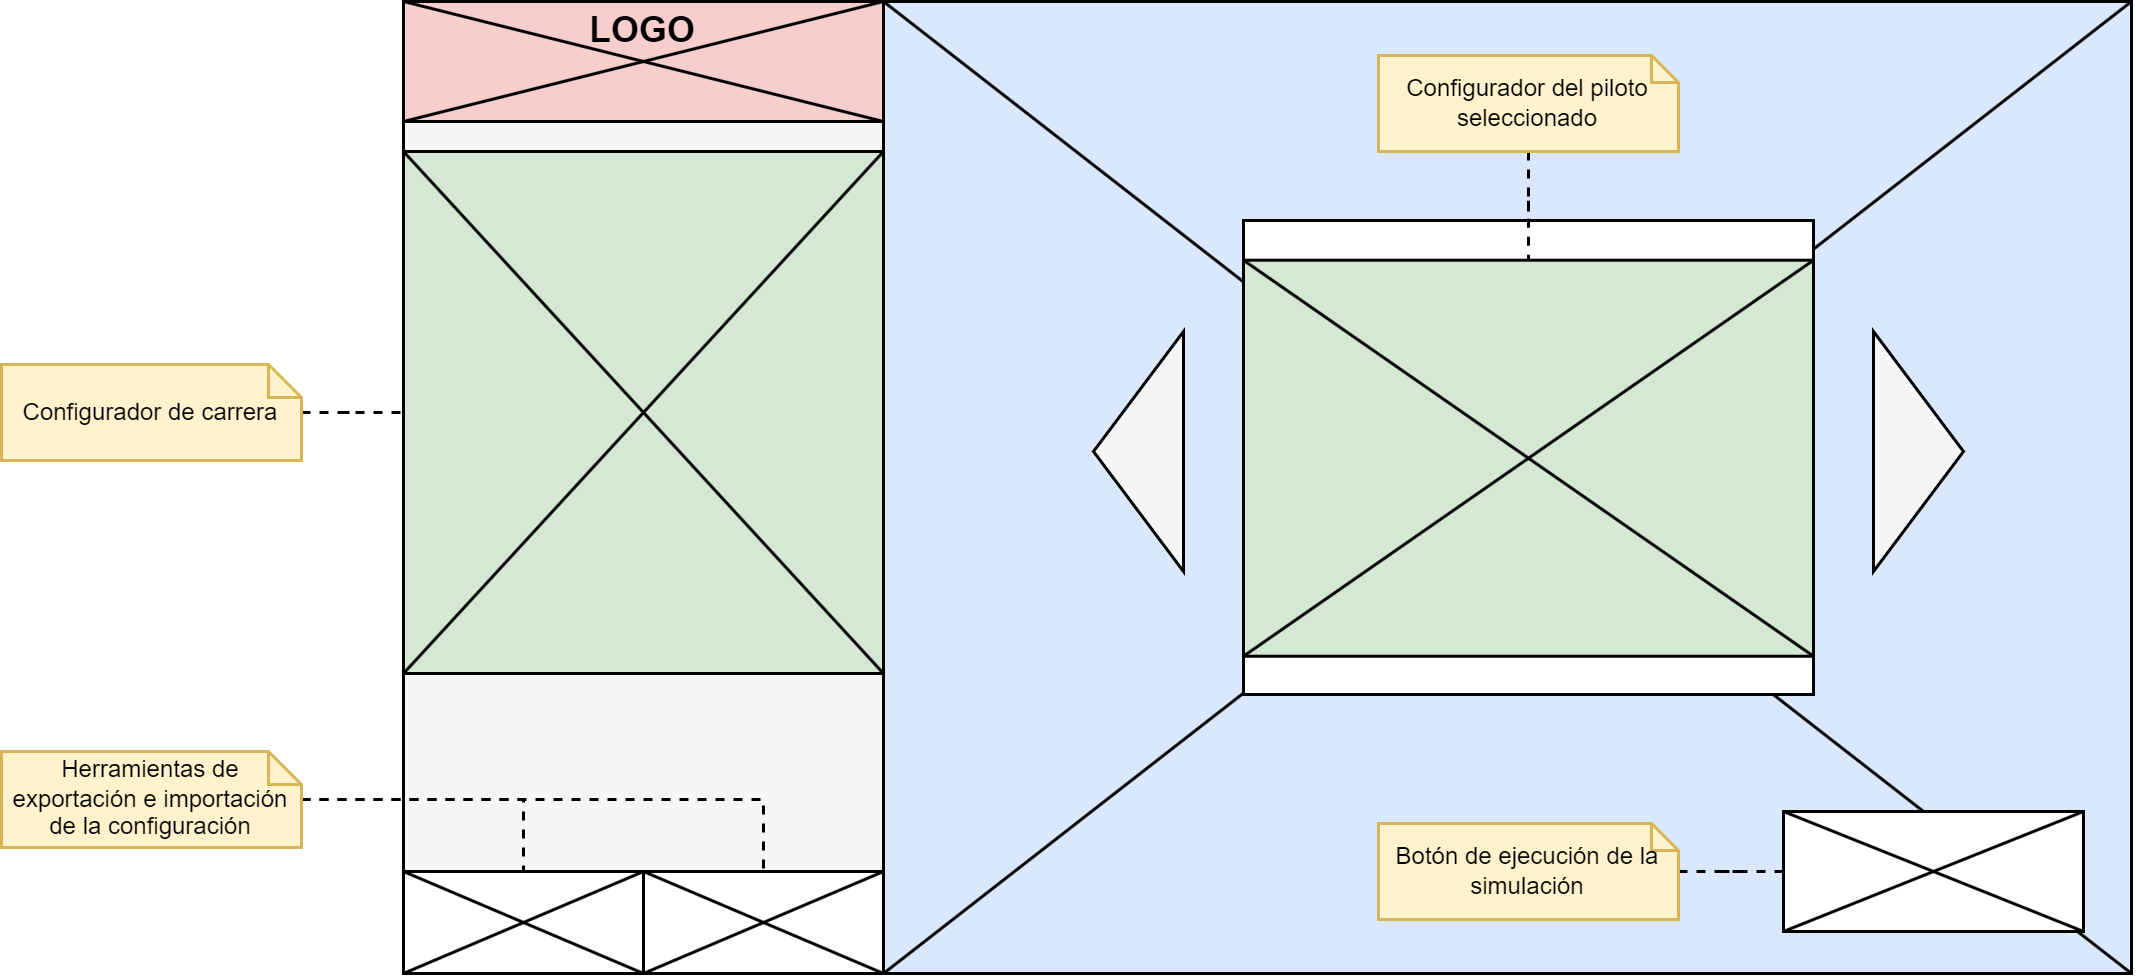
\includegraphics[width=\textwidth]{imagenes/pag1-proto.png}
    \caption{Prototipo del configurador antes de la carrera.}
    \label{fig:protoconfig}
 \end{figure}

 \begin{figure}[H]
    \centering
    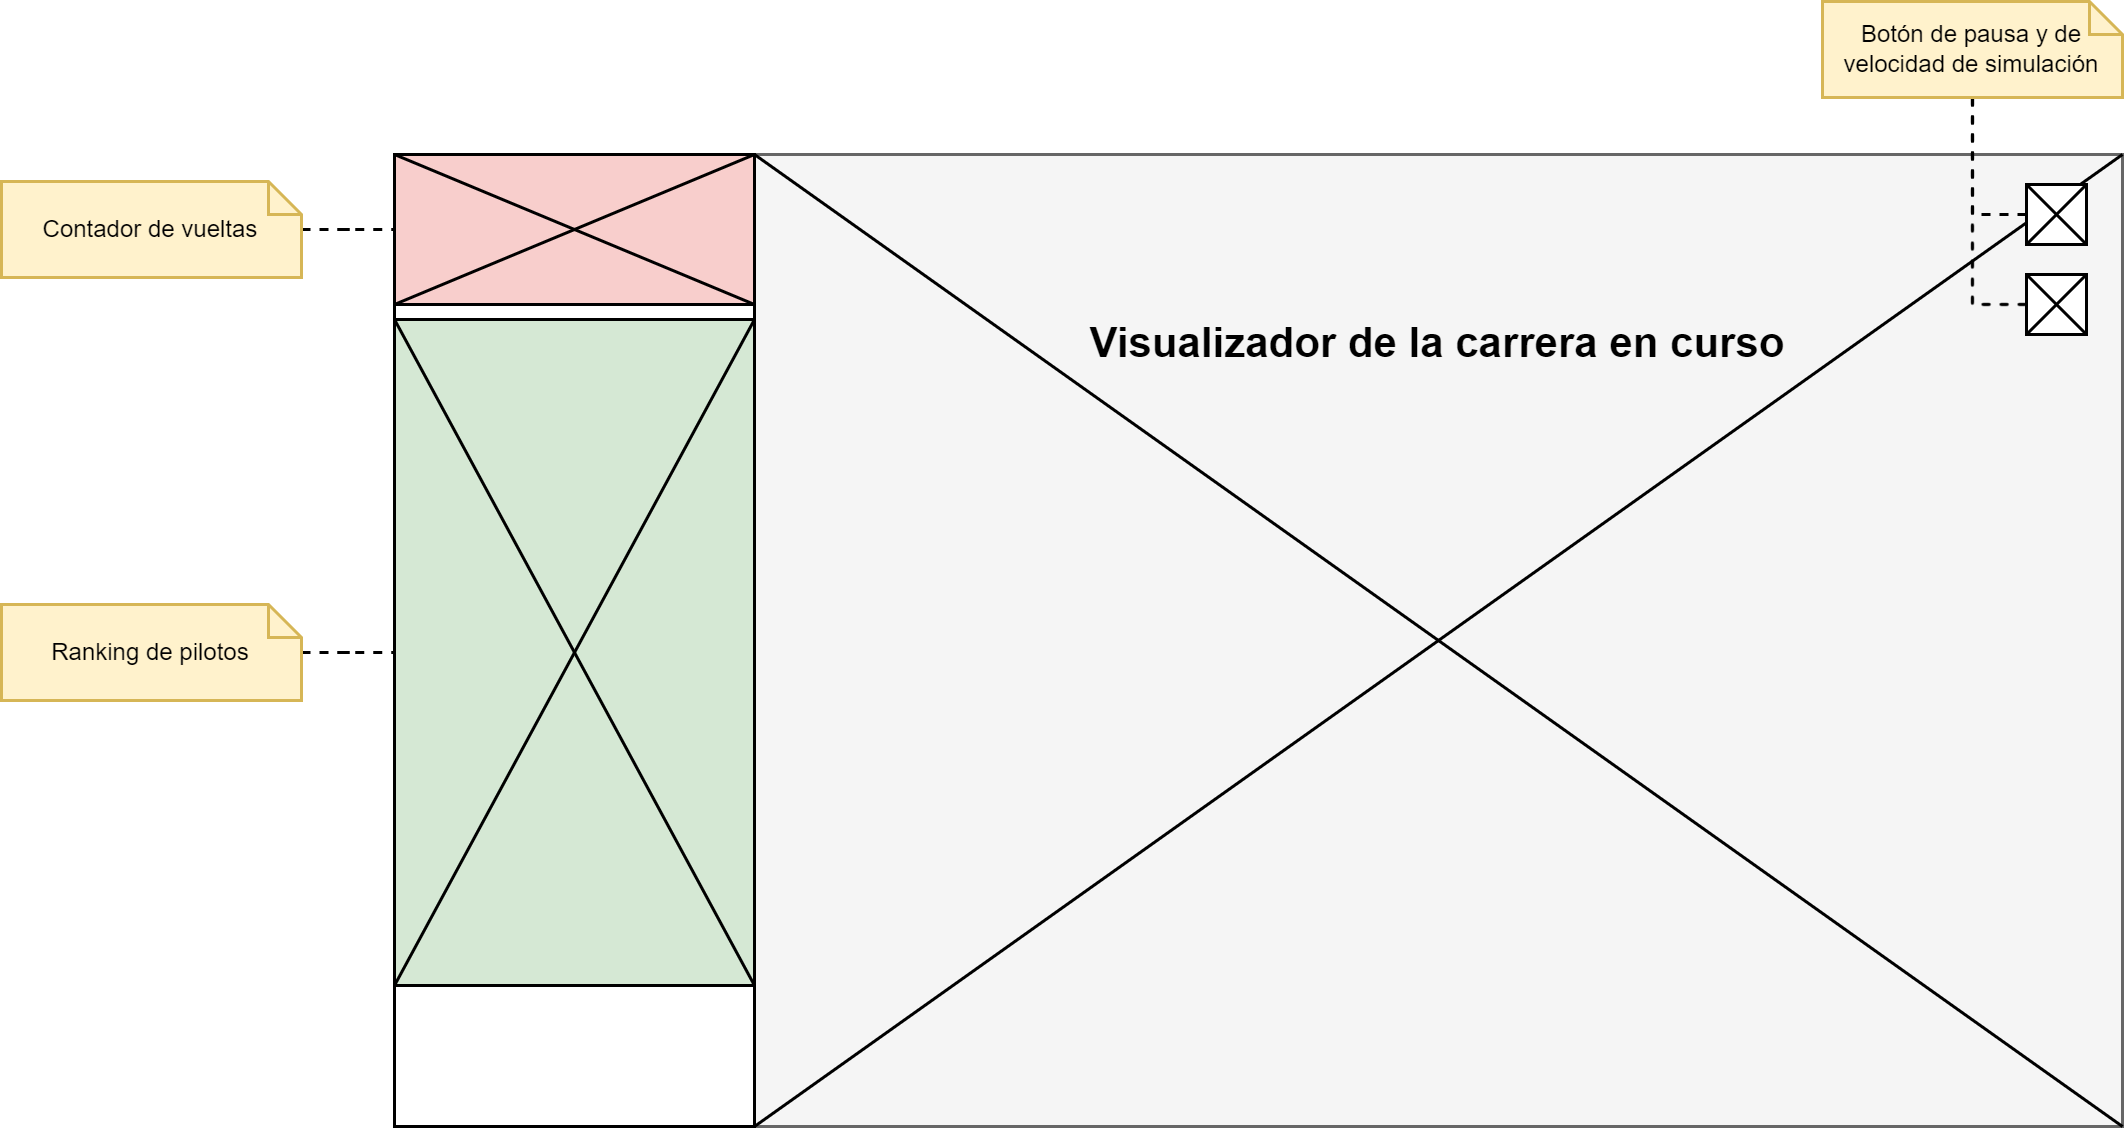
\includegraphics[width=\textwidth]{imagenes/pag2-proto.png}
    \caption{Prototipo de la interfaz de las opciones durante la carrera.}
    \label{fig:protoranking}
 \end{figure}

% DUDAS
% PUSE EXPLICACION GENERAL, PERO NO SE EXACTAMENTE QUE ES
% esto son datos cambiantes, puedo poner algo inicial, pero seguramente haya que modificarlo al final
% no se ni siquiera el numero de sprints que va a haber!! (tendria que tener una velocidad de equipo)
\chapter{Planificación}

\section{Introducción}

Se pretende utilizar una metodología ágil para el desarrollo del proyecto, más concretamente una adaptación de Scrum a las condiciones del mismo, junto a otras herramientas.

\bigskip
% El principal motivo de adaptar Scrum es que
% rescribir
Al ser solo una persona desarrollando el proyecto, es imposible seguir algunas fases del marco de trabajo como \textit{Daily Meetings}, entre otros. Las fases que son aplicables son: \textit{Sprint Planning}. No obstante, todos los artefactos se pueden generar.

\bigskip

Otros aspectos de Scrum que se van a aplicar son: la utilización de sprints para desarrollar el proyecto, su enfoque iterativo e incremental y las Historias de Usuario.

\bigskip

Además, se van a utilizar herramientas que no son estrictamente de metodologías ágiles, como el diagrama de Gantt, para planificar la cantidad de tiempo que se piensa dedicar a cada sprint o Historia de Usuario, dependiendo del nivel de detalle. 

\bigskip

Por último, cabe recordar que no se pretende seguir Scrum de manera precisa, al no cumplir todos los requisitos para poder usarlo. Solo que se piensa usar algunos aspectos aplicables del marco, junto a otras herramientas que no son exactamente de metodologías ágiles.


\section{Product Backlog}

El \textit{Product Backlog} con las Historias de Usuario, ordenadas por prioridad y con sus Puntos de Historia (PH), son:

\begin{table}[H]
    \centering
    \begin{tabularx}{\textwidth}{| >{\centering\arraybackslash}X | >{\centering\arraybackslash}m{5.5cm} | >{\centering\arraybackslash}X | >{\centering\arraybackslash}X |}
        \hline
        \textbf{Código} & \textbf{Descripción} & \textbf{Prioridad} & \textbf{PH} \\
        \hline
        HU1 & Como usuario, quiero que el sistema simula la conducción de varios pilotos en una carrera de coches, simulando adelantamientos y sorteo de obstáculos. & 1 & 5 \\
        \hline
        HU2 & Como usuario, quiero modificar los ajustes de la simulación antes de comenzar la carrera. & 2 & 3 \\
        \hline
        HU3 & Como usuario, quiero modificar el estado de los pilotos durante la carrera. & 2 & 2 \\
        \hline
        HU4 & Como usuario, quiero ver la posición actual de los pilotos de la carrera en curso. & 3 & 3 \\
        \hline
        HU5 & Como usuario, quiero ver el número de vueltas de la carrera en curso. & 3 & 2 \\ 
        \hline
        HU6 & Como usuario, quiero guardar la configuración de una carrera para su posterior uso. & 4 & 2\\
        \hline
        HU7 & Como usuario, quiero cargar la configuración de una carrera almacenada en un archivo. & 4 & 2 \\
        \hline
        HU8 & Como usuario, quiero pausar y reanudar la simulación en curso. & 5 & 0,5 \\
        \hline
        HU9 & Como usuario, quiero modificar la velocidad de la simulación. & 5 & 0,5 \\
        \hline
    \end{tabularx}
\end{table}
    
\section{Velocidad del equipo}

Esto solo es una estimación de la velocidad que se puede alcanzar para el primer Sprint, en función de los puntos de historia realizados al final del mismo se actualizará la velocidad del equipo.

\bigskip

Algunos aspectos a tener en cuenta son:

\begin{itemize}
    \item Duración de los sprints de \sprintLength, que equivalen a \actualSprintLength, quitando fines de semana.
    \item 1 PH representa un día de trabajo ideal a jornada completa (8 horas), pero suponiendo factores externos serán 5 
    horas reales. Usando las horas reales, 1 PH se completaría en 1,6 días.
    % \item Trabajaré 24 horas semanales.
    \item Hay un total de \projectph en el proyecto.
\end{itemize}

\bigskip

Sabiendo esto, la estimación de la velocidad del equipo para la primera iteración es: $\frac{10 \text{ días/sprint}}{1.6 \text{ días/PH}} = 6.25 \text{ PH/sprint} \simeq \mathbf{7\,PH/sprint}$
% $2 \text{ semanas/sprint} \times 20 \text{ horas/semana} \times 8 \text{ horas/PH} = $

\section{Diseño del Sprint}

Este proyecto se dividirá en \sprintNro sprints, cuya duración será de \sprintLength. A continuación se desglosará qué se realizará en cada uno de ellos.

\subsection{Sprint 1}
\begin{itemize}
    \item Explicación: En este sprint se pretende tener la base de la aplicación en funcionamiento. Como base se entiende a que los coches puedan moverse por el mapa mediante el algoritmo de navegación, pudiendo esquivar obstáculos y adelantarse.
    \item Temporización:
    \item Historias de Usuario abordadas: HU1
\end{itemize}

\section{Diagrama de Gantt}

\chapter{Análisis}

En este capítulo se abordará en más detalle cada Historia de Usuario, indicando sus pruebas de validación y las tareas que pueden surgir de cada una de ellas.

\bigskip

Cabe destacar que el campo de ``Entrega'' indica en qué sprint se va a realizar, mientras que el campo de ``Estimación'' indica cuanto Puntos de Historia (PH) se le han asignado.

\bigskip

Cada Historia de Usuario se desarrollará en una tabla a continuación:

% \section{Historias de Usuario divididas en subtareas}



% \begin{table}[H]
%     \begin{tabularx}{\textwidth}{| X | X | X |}
%         \hline
%         \multicolumn{1}{|l|}{\textbf{Identificador:} HU1} & \multicolumn{2}{l|}{Algoritmo de navegación.}
%         \\ \hline
%         \multicolumn{3}{|>{\hsize=\dimexpr3\hsize+4\tabcolsep+2\arrayrulewidth\relax\linewidth=\hsize}X|}{\textbf{Descripción:} Como usuario, quiero que el sistema simule la conducción de varios pilotos en una carrera de coches, incluyendo adelantamientos y sorteo de obstáculos.}
%         \\ \hline
%         \textbf{Estimación:} 5 & \textbf{Prioridad:} 1 & \textbf{Entrega:} 1
%         \\ \hline
%         \multicolumn{3}{|>{\hsize=\dimexpr3\hsize+4\tabcolsep+2\arrayrulewidth\relax\linewidth=\hsize}X|}{\textbf{Tareas:}
%         \begin{itemize}
%             \item Implementar el controlador del volante de los vehículos, de manera que sean capaces de seguir una ruta de forma suave.
%             \item Implementar la malla de navegación.
%             \item Implementar el algoritmo a partir de la malla.
%             \item Implementar la lógica de los vehículos, de forma que sean capaces usar esta malla para tomar decisiones.
%         \end{itemize}
%         }
%         \\ \hline
%         \multicolumn{3}{|>{\hsize=\dimexpr3\hsize+4\tabcolsep+2\arrayrulewidth\relax\linewidth=\hsize}X|}{\textbf{Requisitos relacionados:} RF6, RNF4.}
%         \\ \hline
%         \multicolumn{3}{|>{\hsize=\dimexpr3\hsize+4\tabcolsep+2\arrayrulewidth\relax\linewidth=\hsize}X|}{\textbf{Pruebas de aceptación:}
%         \begin{itemize}
%             \item Los pilotos deben ser capaces de esquivar obstáculos en la pista.
%             \item La simulación debe poder ejecutarse en un tiempo razonable, de manera que se pueda seguir la carrera en tiempo real.
%             \item Los pilotos deben ser capaces de adelantar a otros que sean más lentos sin provocar accidentes.
%         \end{itemize}
%         }
%         \\ \hline
%         \multicolumn{3}{|>{\hsize=\dimexpr3\hsize+4\tabcolsep+2\arrayrulewidth\relax\linewidth=\hsize}X|}{\textbf{Observaciones:}}
%         \\ \hline
%     \end{tabularx}
% \end{table}

% \begin{table}[H]
%     \begin{tabularx}{\textwidth}{| X | X | X |}
%         \hline
%         \multicolumn{1}{|l|}{\textbf{Identificador:} HU1} & \multicolumn{2}{l|}{lorem ipsum dolor sit amet.}
%         \\ \hline
%         \multicolumn{3}{|>{\hsize=\dimexpr3\hsize+4\tabcolsep+2\arrayrulewidth\relax\linewidth=\hsize}X|}{\textbf{Descripción:} lorem ipsum dolor sit amet.}
%         \\ \hline
%         \textbf{Estimación:} X & \textbf{Prioridad:} X & \textbf{Entrega:} X
%         \\ \hline
%         \multicolumn{3}{|>{\hsize=\dimexpr3\hsize+4\tabcolsep+2\arrayrulewidth\relax\linewidth=\hsize}X|}{\textbf{Tareas:}
%         \begin{itemize}
%             \item Roma no se hizo en un día.
%         \end{itemize}
%         }
%         \\ \hline
%         \multicolumn{3}{|>{\hsize=\dimexpr3\hsize+4\tabcolsep+2\arrayrulewidth\relax\linewidth=\hsize}X|}{\textbf{Requisitos relacionados:} RF6, RNF4.}
%         \\ \hline
%         \multicolumn{3}{|>{\hsize=\dimexpr3\hsize+4\tabcolsep+2\arrayrulewidth\relax\linewidth=\hsize}X|}{\textbf{Pruebas de aceptación:}
%         \begin{itemize}
%             \item Algo tangible.
%         \end{itemize}
%         }
%         \\ \hline
%         \multicolumn{3}{|>{\hsize=\dimexpr3\hsize+4\tabcolsep+2\arrayrulewidth\relax\linewidth=\hsize}X|}{\textbf{Observaciones:}}
%         \\ \hline
%     \end{tabularx}
% \end{table}

\begin{table}[H]
    \begin{tabularx}{\textwidth}{| X | X | X |}
        \hline
        \multicolumn{1}{|l|}{\textbf{Identificador:} HU1} & \multicolumn{2}{l|}{Modelado de los coches y circuito.}
        \\ \hline
        \multicolumn{3}{|>{\hsize=\dimexpr3\hsize+4\tabcolsep+2\arrayrulewidth\relax\linewidth=\hsize}X|}{\textbf{Descripción:} Como usuario, quiero tener una representación en 3D de los coches y el circuito.}
        \\ \hline
        \textbf{Estimación:} 3 & \textbf{Prioridad:} 1 & \textbf{Entrega:} 4
        \\ \hline
        \multicolumn{3}{|>{\hsize=\dimexpr3\hsize+4\tabcolsep+2\arrayrulewidth\relax\linewidth=\hsize}X|}{\textbf{Tareas:}
        \begin{itemize}
            \item Modelar el trazado del circuito.
            \item Modelar los vehículos, o en su defecto, obtener modelos ya hechos.
        \end{itemize}
        }
        \\ \hline
        \multicolumn{3}{|>{\hsize=\dimexpr3\hsize+4\tabcolsep+2\arrayrulewidth\relax\linewidth=\hsize}X|}{\textbf{Requisitos relacionados:}}
        \\ \hline
        \multicolumn{3}{|>{\hsize=\dimexpr3\hsize+4\tabcolsep+2\arrayrulewidth\relax\linewidth=\hsize}X|}{\textbf{Pruebas de aceptación:}
        }
        \\ \hline
        \multicolumn{3}{|>{\hsize=\dimexpr3\hsize+4\tabcolsep+2\arrayrulewidth\relax\linewidth=\hsize}X|}{\textbf{Observaciones:}}
        \\ \hline
    \end{tabularx}
\end{table}

\begin{table}[H]
    \begin{tabularx}{\textwidth}{| X | X | X |}
        \hline
        \multicolumn{1}{|l|}{\textbf{Identificador:} HU2} & \multicolumn{2}{l|}{Cálculo de ruta óptima en el circuito.}
        \\ \hline
        \multicolumn{3}{|>{\hsize=\dimexpr3\hsize+4\tabcolsep+2\arrayrulewidth\relax\linewidth=\hsize}X|}{\textbf{Descripción:} Como usuario, quiero que los pilotos calculen la ruta más óptima en el circuito.}
        \\ \hline
        \textbf{Estimación:} 8 & \textbf{Prioridad:} 1 & \textbf{Entrega:} 5
        \\ \hline
        \multicolumn{3}{|>{\hsize=\dimexpr3\hsize+4\tabcolsep+2\arrayrulewidth\relax\linewidth=\hsize}X|}{\textbf{Tareas:}
        \begin{itemize}
            \item Implementar la malla de navegación, para que los coches puedan calcular rutas.
            \item Implementar el algoritmo de navegación, que haga uso de la malla.
            \item Crear los objetos auxiliares, para indicar a la malla la ruta más rápida.
        \end{itemize}
        }
        \\ \hline
        \multicolumn{3}{|>{\hsize=\dimexpr3\hsize+4\tabcolsep+2\arrayrulewidth\relax\linewidth=\hsize}X|}{\textbf{Requisitos relacionados:} RF6, RNF4.}
        \\ \hline
        \multicolumn{3}{|>{\hsize=\dimexpr3\hsize+4\tabcolsep+2\arrayrulewidth\relax\linewidth=\hsize}X|}{\textbf{Pruebas de aceptación:}
        \begin{itemize}
            \item El algoritmo debe calcular una ruta que no dé la vuelta en el circuito.
            \item El algoritmo debe obtener un resultado en un tiempo razonable.
        \end{itemize}
        }
        \\ \hline
        \multicolumn{3}{|>{\hsize=\dimexpr3\hsize+4\tabcolsep+2\arrayrulewidth\relax\linewidth=\hsize}X|}{\textbf{Observaciones:}}
        \\ \hline
    \end{tabularx}
\end{table}

\begin{table}[H]
    \begin{tabularx}{\textwidth}{| X | X | X |}
        \hline
        \multicolumn{1}{|l|}{\textbf{Identificador:} HU3} & \multicolumn{2}{l|}{Seguimiento de una ruta con el volante.}
        \\ \hline
        \multicolumn{3}{|>{\hsize=\dimexpr3\hsize+4\tabcolsep+2\arrayrulewidth\relax\linewidth=\hsize}X|}{\textbf{Descripción:} Como usuario, quiero que los pilotos sean capaces de seguir una ruta de manera suave.}
        \\ \hline
        \textbf{Estimación:} 5 & \textbf{Prioridad:} 1 & \textbf{Entrega:} 4
        \\ \hline
        \multicolumn{3}{|>{\hsize=\dimexpr3\hsize+4\tabcolsep+2\arrayrulewidth\relax\linewidth=\hsize}X|}{\textbf{Tareas:}
        \begin{itemize}
            \item Implementar el controlador PID para usarlo en el volante.
            \item Implementar un algoritmo para obtener el mejor valor de las constantes.
        \end{itemize}
        }
        \\ \hline
        \multicolumn{3}{|>{\hsize=\dimexpr3\hsize+4\tabcolsep+2\arrayrulewidth\relax\linewidth=\hsize}X|}{\textbf{Requisitos relacionados:} RF6, RNF4.}
        \\ \hline
        \multicolumn{3}{|>{\hsize=\dimexpr3\hsize+4\tabcolsep+2\arrayrulewidth\relax\linewidth=\hsize}X|}{\textbf{Dependencias:} HU2.}
        \\ \hline   
        \multicolumn{3}{|>{\hsize=\dimexpr3\hsize+4\tabcolsep+2\arrayrulewidth\relax\linewidth=\hsize}X|}{\textbf{Pruebas de aceptación:}
        \begin{itemize}
            \item La amplitud de las oscilaciones del vehículo en línea recta deben tener un tamaño menor a la anchura del coche.
            \item El coche debe tomar la curvas de manera suave.
        \end{itemize}
        }
        \\ \hline
        \multicolumn{3}{|>{\hsize=\dimexpr3\hsize+4\tabcolsep+2\arrayrulewidth\relax\linewidth=\hsize}X|}{\textbf{Observaciones:} El algoritmo utilizado para ajustar los valores del PID ha sido un algoritmo genético.}
        \\ \hline
    \end{tabularx}
\end{table}

\begin{table}[H]
    \begin{tabularx}{\textwidth}{| X | X | X |}
        \hline
        \multicolumn{1}{|l|}{\textbf{Identificador:} HU4} & \multicolumn{2}{l|}{Adelantamiento entre vehículos.}
        \\ \hline
        \multicolumn{3}{|>{\hsize=\dimexpr3\hsize+4\tabcolsep+2\arrayrulewidth\relax\linewidth=\hsize}X|}{\textbf{Descripción:} Como usuario, quiero que los pilotos sean capaces de adelantarse entre ellos.}
        \\ \hline
        \textbf{Estimación:} 5 & \textbf{Prioridad:} 1 & \textbf{Entrega:} 6
        \\ \hline
        \multicolumn{3}{|>{\hsize=\dimexpr3\hsize+4\tabcolsep+2\arrayrulewidth\relax\linewidth=\hsize}X|}{\textbf{Tareas:}
        \begin{itemize}
            \item Haciendo uso del algoritmo de HU2, implementar la lógica necesaria para saber cuando recalcular la ruta.
            \item Ajustar las colisiones de los vehículos, de forma que tengan espacio para adelantar.
        \end{itemize}
        }
        \\ \hline
        \multicolumn{3}{|>{\hsize=\dimexpr3\hsize+4\tabcolsep+2\arrayrulewidth\relax\linewidth=\hsize}X|}{\textbf{Requisitos relacionados:} RF6, RNF4.}
        \\ \hline
        \multicolumn{3}{|>{\hsize=\dimexpr3\hsize+4\tabcolsep+2\arrayrulewidth\relax\linewidth=\hsize}X|}{\textbf{Dependencias:} HU2.}
        \\ \hline   
        \multicolumn{3}{|>{\hsize=\dimexpr3\hsize+4\tabcolsep+2\arrayrulewidth\relax\linewidth=\hsize}X|}{\textbf{Pruebas de aceptación:}
        \begin{itemize}
            \item El adelantamiento de un coche a otro no debe provocar el accidente de ninguno de los dos.
        \end{itemize}
        }
        \\ \hline
        \multicolumn{3}{|>{\hsize=\dimexpr3\hsize+4\tabcolsep+2\arrayrulewidth\relax\linewidth=\hsize}X|}{\textbf{Observaciones:}}
        \\ \hline
    \end{tabularx}
\end{table}

\begin{table}[H]
    \begin{tabularx}{\textwidth}{| X | X | X |}
        \hline
        \multicolumn{1}{|l|}{\textbf{Identificador:} HU5} & \multicolumn{2}{l|}{Maniobra de recuperación en accidentes.}
        \\ \hline
        \multicolumn{3}{|>{\hsize=\dimexpr3\hsize+4\tabcolsep+2\arrayrulewidth\relax\linewidth=\hsize}X|}{\textbf{Descripción:} Como usuario, quiero que los pilotos sean capaces de recuperarse después de un accidente.}
        \\ \hline
        \textbf{Estimación:} 3 & \textbf{Prioridad:} 1 & \textbf{Entrega:} 6
        \\ \hline
        \multicolumn{3}{|>{\hsize=\dimexpr3\hsize+4\tabcolsep+2\arrayrulewidth\relax\linewidth=\hsize}X|}{\textbf{Tareas:}
        \begin{itemize}
            \item Implementar la lógica para que los pilotos recalculen una ruta que les devuelva a la pista utilizando el algoritmo de navegación.
        \end{itemize}
        }
        \\ \hline
        \multicolumn{3}{|>{\hsize=\dimexpr3\hsize+4\tabcolsep+2\arrayrulewidth\relax\linewidth=\hsize}X|}{\textbf{Requisitos relacionados:} RF6, RNF4.}
        \\ \hline
        \multicolumn{3}{|>{\hsize=\dimexpr3\hsize+4\tabcolsep+2\arrayrulewidth\relax\linewidth=\hsize}X|}{\textbf{Dependencias:} HU2.}
        \\ \hline        
        \multicolumn{3}{|>{\hsize=\dimexpr3\hsize+4\tabcolsep+2\arrayrulewidth\relax\linewidth=\hsize}X|}{\textbf{Pruebas de aceptación:}
        \begin{itemize}
            \item La nueva ruta debe calcularse en un tiempo razonable, de manera que pueda hacerse en tiempo real.
        \end{itemize}
        }
        \\ \hline
        \multicolumn{3}{|>{\hsize=\dimexpr3\hsize+4\tabcolsep+2\arrayrulewidth\relax\linewidth=\hsize}X|}{\textbf{Observaciones:}}
        \\ \hline
    \end{tabularx}
\end{table}

% ANTIGUOS DEL SPRINT 4

\begin{table}[H]
    \begin{tabularx}{\textwidth}{| X | X | X |}
        \hline
        \multicolumn{1}{|l|}{\textbf{Identificador:} HU6} & \multicolumn{2}{l|}{Modificación de ajustes antes de la carrera.}
        \\ \hline
        \multicolumn{3}{|>{\hsize=\dimexpr3\hsize+4\tabcolsep+2\arrayrulewidth\relax\linewidth=\hsize}X|}{\textbf{Descripción:} Como usuario, quiero modificar los ajustes de la simulación antes de comenzar la carrera.}
        \\ \hline
        \textbf{Estimación:} 2 & \textbf{Prioridad:} 2 & \textbf{Entrega:} 7
        \\ \hline
        \multicolumn{3}{|>{\hsize=\dimexpr3\hsize+4\tabcolsep+2\arrayrulewidth\relax\linewidth=\hsize}X|}{\textbf{Tareas:}
        \begin{itemize}
            \item Implementar los deslizadores correspondientes al número de vueltas, de coches, hora, aguante y experiencia.
            \item Implementar los campos de texto para el nombre y los apellidos.
            \item Programar la lógica necesaria para que los coches aparezcan en las posiciones correctas.
            \item Programar la lógica de las flechas para elegir a los pilotos.
        \end{itemize}
        }
        \\ \hline
        \multicolumn{3}{|>{\hsize=\dimexpr3\hsize+4\tabcolsep+2\arrayrulewidth\relax\linewidth=\hsize}X|}{\textbf{Requisitos relacionados:} RF1, RNF2, RNF3.}
        \\ \hline
        \multicolumn{3}{|>{\hsize=\dimexpr3\hsize+4\tabcolsep+2\arrayrulewidth\relax\linewidth=\hsize}X|}{\textbf{Pruebas de aceptación:}
        \begin{itemize}
            % \item No se podrá elegir un número menor de 1 para la cantidad de vueltas.
            % \item No se podrá elegir un número menor de 2 coches.
            \item No se podrá dejar el campo del nombre y los apellidos vacíos.
        \end{itemize}
        }
        \\ \hline
        \multicolumn{3}{|>{\hsize=\dimexpr3\hsize+4\tabcolsep+2\arrayrulewidth\relax\linewidth=\hsize}X|}{\textbf{Observaciones:}}
        \\ \hline
    \end{tabularx}
\end{table}

\begin{table}[H]
    \begin{tabularx}{\textwidth}{| X | X | X |}
        \hline
        \multicolumn{1}{|l|}{\textbf{Identificador:} HU7} & \multicolumn{2}{l|}{Modificación del estado de los pilotos.}
        \\ \hline
        \multicolumn{3}{|>{\hsize=\dimexpr3\hsize+4\tabcolsep+2\arrayrulewidth\relax\linewidth=\hsize}X|}{\textbf{Descripción:} Como usuario, quiero modificar el estado de los pilotos durante la carrera.}
        \\ \hline
        \textbf{Estimación:} 2 & \textbf{Prioridad:} 2 & \textbf{Entrega:} 7
        \\ \hline
        \multicolumn{3}{|>{\hsize=\dimexpr3\hsize+4\tabcolsep+2\arrayrulewidth\relax\linewidth=\hsize}X|}{\textbf{Tareas:}
        \begin{itemize}
            \item Implementar los deslizadores referentes al aguante físico y mental y la agresividad.
        \end{itemize}
        }
        \\ \hline
        \multicolumn{3}{|>{\hsize=\dimexpr3\hsize+4\tabcolsep+2\arrayrulewidth\relax\linewidth=\hsize}X|}{\textbf{Requisitos relacionados:} RF3, RNF5.}
        \\ \hline
        \multicolumn{3}{|>{\hsize=\dimexpr3\hsize+4\tabcolsep+2\arrayrulewidth\relax\linewidth=\hsize}X|}{\textbf{Dependencias:} HU4.}        
        \\ \hline
        \multicolumn{3}{|>{\hsize=\dimexpr3\hsize+4\tabcolsep+2\arrayrulewidth\relax\linewidth=\hsize}X|}{\textbf{Pruebas de aceptación:}
        \begin{itemize}
            \item Los cambios en el estado deberán verse reflejados en el comportamiento del piloto seleccionado durante la carrera.
        \end{itemize}
        }
        \\ \hline
        \multicolumn{3}{|>{\hsize=\dimexpr3\hsize+4\tabcolsep+2\arrayrulewidth\relax\linewidth=\hsize}X|}{\textbf{Observaciones:}}
        \\ \hline
    \end{tabularx}
\end{table}


\begin{table}[H]
    \begin{tabularx}{\textwidth}{| X | X | X |}
        \hline
        \multicolumn{1}{|l|}{\textbf{Identificador:} HU8} & \multicolumn{2}{l|}{Visualización de la información de los pilotos.}
        \\ \hline
        \multicolumn{3}{|>{\hsize=\dimexpr3\hsize+4\tabcolsep+2\arrayrulewidth\relax\linewidth=\hsize}X|}{\textbf{Descripción:} Como usuario, quiero ver la posición actual y el estado de los pilotos de la carrera en curso.}
        \\ \hline
        \textbf{Estimación:} 3 & \textbf{Prioridad:} 3 & \textbf{Entrega:} 7
        \\ \hline
        \multicolumn{3}{|>{\hsize=\dimexpr3\hsize+4\tabcolsep+2\arrayrulewidth\relax\linewidth=\hsize}X|}{\textbf{Tareas:}
        \begin{itemize}
            \item Implementar el panel de las posiciones y el estado.
            \item Implementar la lógica asociada al cálculo de la posición general de cada piloto.
            \item Implementar la funcionalidad de mostrar los deslizadores del piloto al pulsar.
        \end{itemize}
        }
        \\ \hline
        \multicolumn{3}{|>{\hsize=\dimexpr3\hsize+4\tabcolsep+2\arrayrulewidth\relax\linewidth=\hsize}X|}{\textbf{Requisitos relacionados:} RF2, RNF3.}
        \\ \hline
        \multicolumn{3}{|>{\hsize=\dimexpr3\hsize+4\tabcolsep+2\arrayrulewidth\relax\linewidth=\hsize}X|}{\textbf{Pruebas de aceptación:}
        \begin{itemize}
            \item Cuando un piloto cambie posiciones con otro, la lista de posiciones de los pilotos debe cambiar.
            \item El cambio del estado del piloto producido por la carrera será reflejado en el deslizador.
        \end{itemize}
        }
        \\ \hline
        \multicolumn{3}{|>{\hsize=\dimexpr3\hsize+4\tabcolsep+2\arrayrulewidth\relax\linewidth=\hsize}X|}{\textbf{Observaciones:}}
        \\ \hline
    \end{tabularx}
\end{table}

\begin{table}[H]
    \begin{tabularx}{\textwidth}{| X | X | X |}
        \hline
        \multicolumn{1}{|l|}{\textbf{Identificador:} HU9} & \multicolumn{2}{l|}{Visualización de las vueltas restantes.}
        \\ \hline
        \multicolumn{3}{|>{\hsize=\dimexpr3\hsize+4\tabcolsep+2\arrayrulewidth\relax\linewidth=\hsize}X|}{\textbf{Descripción:} Como usuario, quiero ver el número de vueltas de la carrera en curso.}
        \\ \hline
        \textbf{Estimación:} 2 & \textbf{Prioridad:} 3 & \textbf{Entrega:} 8
        \\ \hline
        \multicolumn{3}{|>{\hsize=\dimexpr3\hsize+4\tabcolsep+2\arrayrulewidth\relax\linewidth=\hsize}X|}{\textbf{Tareas:}
        \begin{itemize}
            \item Implementar la lógica para calcular la vuelta actual.
            \item Crear el contador de la interfaz que mostrará las vueltas.
        \end{itemize}
        }
        \\ \hline
        \multicolumn{3}{|>{\hsize=\dimexpr3\hsize+4\tabcolsep+2\arrayrulewidth\relax\linewidth=\hsize}X|}{\textbf{Requisitos relacionados:} RF9, RNF3.}
        \\ \hline
        \multicolumn{3}{|>{\hsize=\dimexpr3\hsize+4\tabcolsep+2\arrayrulewidth\relax\linewidth=\hsize}X|}{\textbf{Pruebas de aceptación:}
        \begin{itemize}
            \item El marcador no deberá mostrar como vuelta actual el número 0 ni un número superior al número máximo.
        \end{itemize}
        }
        \\ \hline
        \multicolumn{3}{|>{\hsize=\dimexpr3\hsize+4\tabcolsep+2\arrayrulewidth\relax\linewidth=\hsize}X|}{\textbf{Observaciones:}}
        \\ \hline
    \end{tabularx}
\end{table}


\begin{table}[H]
    \begin{tabularx}{\textwidth}{| X | X | X |}
        \hline
        \multicolumn{1}{|l|}{\textbf{Identificador:} HU10} & \multicolumn{2}{l|}{Exportación de la configuración.}
        \\ \hline
        \multicolumn{3}{|>{\hsize=\dimexpr3\hsize+4\tabcolsep+2\arrayrulewidth\relax\linewidth=\hsize}X|}{\textbf{Descripción:} Como usuario, quiero guardar la configuración de una carrera para su posterior uso.}
        \\ \hline
        \textbf{Estimación:} 2 & \textbf{Prioridad:} 4 & \textbf{Entrega:} 8
        \\ \hline
        \multicolumn{3}{|>{\hsize=\dimexpr3\hsize+4\tabcolsep+2\arrayrulewidth\relax\linewidth=\hsize}X|}{\textbf{Tareas:}
        \begin{itemize}
            \item Implementar la lógica referente a la escritura de la configuración en un archivo externo.
        \end{itemize}
        }
        \\ \hline
        \multicolumn{3}{|>{\hsize=\dimexpr3\hsize+4\tabcolsep+2\arrayrulewidth\relax\linewidth=\hsize}X|}{\textbf{Requisitos relacionados:} RF7.}
        \\ \hline
        \multicolumn{3}{|>{\hsize=\dimexpr3\hsize+4\tabcolsep+2\arrayrulewidth\relax\linewidth=\hsize}X|}{\textbf{Pruebas de aceptación:}
        \begin{itemize}
            \item Al pulsar el botón se debe producir un fichero externo con la configuración exacta que había en el momento.
        \end{itemize}
        }
        \\ \hline
        \multicolumn{3}{|>{\hsize=\dimexpr3\hsize+4\tabcolsep+2\arrayrulewidth\relax\linewidth=\hsize}X|}{\textbf{Observaciones:}}
        \\ \hline
    \end{tabularx}
\end{table}

\begin{table}[H]
    \begin{tabularx}{\textwidth}{| X | X | X |}
        \hline
        \multicolumn{1}{|l|}{\textbf{Identificador:} HU11} & \multicolumn{2}{l|}{Importación de la configuración.}
        \\ \hline
        \multicolumn{3}{|>{\hsize=\dimexpr3\hsize+4\tabcolsep+2\arrayrulewidth\relax\linewidth=\hsize}X|}{\textbf{Descripción:} Como usuario, quiero cargar la configuración de una carrera almacenada en un archivo.}
        \\ \hline
        \textbf{Estimación:} 2 & \textbf{Prioridad:} 4 & \textbf{Entrega:} 8
        \\ \hline
        \multicolumn{3}{|>{\hsize=\dimexpr3\hsize+4\tabcolsep+2\arrayrulewidth\relax\linewidth=\hsize}X|}{\textbf{Tareas:}
        \begin{itemize}
            \item Implementar la lógica referente a la modificación de los parámetros por los valores que se encuentren en el archivo.
        \end{itemize}
        }
        \\ \hline
        \multicolumn{3}{|>{\hsize=\dimexpr3\hsize+4\tabcolsep+2\arrayrulewidth\relax\linewidth=\hsize}X|}{\textbf{Requisitos relacionados:} RF8.}
        \\ \hline
        \multicolumn{3}{|>{\hsize=\dimexpr3\hsize+4\tabcolsep+2\arrayrulewidth\relax\linewidth=\hsize}X|}{\textbf{Pruebas de aceptación:}
        \begin{itemize}
            % \item El fichero generado en la fase de exportación debe ser legible por la aplicación.
            \item Ante un fichero válido de configuración, la aplicación lo leerá correctamente y modificará los parámetros de forma adecuada.
        \end{itemize}
        }
        \\ \hline
        \multicolumn{3}{|>{\hsize=\dimexpr3\hsize+4\tabcolsep+2\arrayrulewidth\relax\linewidth=\hsize}X|}{\textbf{Observaciones:}}
        \\ \hline
    \end{tabularx}
\end{table}


\begin{table}[H]
    \begin{tabularx}{\textwidth}{| X | X | X |}
        \hline
        \multicolumn{1}{|l|}{\textbf{Identificador:} HU12} & \multicolumn{2}{l|}{Pausado y reanudación de la simulación.}
        \\ \hline
        \multicolumn{3}{|>{\hsize=\dimexpr3\hsize+4\tabcolsep+2\arrayrulewidth\relax\linewidth=\hsize}X|}{\textbf{Descripción:} Como usuario, quiero pausar y reanudar la simulación en curso.}
        \\ \hline
        \textbf{Estimación:} 0,5 & \textbf{Prioridad:} 5 & \textbf{Entrega:} 8
        \\ \hline
        \multicolumn{3}{|>{\hsize=\dimexpr3\hsize+4\tabcolsep+2\arrayrulewidth\relax\linewidth=\hsize}X|}{\textbf{Tareas:}
        \begin{itemize}
            \item Incluir el botón en la interfaz.
            \item Implementar la lógica relacionada con el botón y el pausado de la simulación.
        \end{itemize}
        }
        \\ \hline
        \multicolumn{3}{|>{\hsize=\dimexpr3\hsize+4\tabcolsep+2\arrayrulewidth\relax\linewidth=\hsize}X|}{\textbf{Requisitos relacionados:} RF5, RNF2.}
        \\ \hline
        \multicolumn{3}{|>{\hsize=\dimexpr3\hsize+4\tabcolsep+2\arrayrulewidth\relax\linewidth=\hsize}X|}{\textbf{Pruebas de aceptación:}
        \begin{itemize}
            \item Al pulsar el botón, debe alternar entre pausado y reanudado.
            \item Al encontrarse la simulación pausada, no se podrá modificar su velocidad.
        \end{itemize}
        }
        \\ \hline
        \multicolumn{3}{|>{\hsize=\dimexpr3\hsize+4\tabcolsep+2\arrayrulewidth\relax\linewidth=\hsize}X|}{\textbf{Observaciones:}}
        \\ \hline
    \end{tabularx}
\end{table}

\begin{table}[H]
    \begin{tabularx}{\textwidth}{| X | X | X |}
        \hline
        \multicolumn{1}{|l|}{\textbf{Identificador:} HU13} & \multicolumn{2}{l|}{Modificación de la velocidad de la simulación.}
        \\ \hline
        \multicolumn{3}{|>{\hsize=\dimexpr3\hsize+4\tabcolsep+2\arrayrulewidth\relax\linewidth=\hsize}X|}{\textbf{Descripción:} Como usuario, quiero modificar la velocidad de la simulación.}
        \\ \hline
        \textbf{Estimación:} 0,5 & \textbf{Prioridad:} 5 & \textbf{Entrega:} 8
        \\ \hline
        \multicolumn{3}{|>{\hsize=\dimexpr3\hsize+4\tabcolsep+2\arrayrulewidth\relax\linewidth=\hsize}X|}{\textbf{Tareas:}
        \begin{itemize}
            \item Incluir el botón en la interfaz.
            \item Implementar la lógica relacionada con el botón y la modificación de la velocidad de simulación.
        \end{itemize}
        }
        \\ \hline
        \multicolumn{3}{|>{\hsize=\dimexpr3\hsize+4\tabcolsep+2\arrayrulewidth\relax\linewidth=\hsize}X|}{\textbf{Requisitos relacionados:} RF4, RNF2.}
        \\ \hline
        \multicolumn{3}{|>{\hsize=\dimexpr3\hsize+4\tabcolsep+2\arrayrulewidth\relax\linewidth=\hsize}X|}{\textbf{Pruebas de aceptación:}
        \begin{itemize}
            \item Al pulsar el botón, debe alternar entre el conjunto de velocidades de simulación existentes.
            \item Este botón no deberá funcionar si la simulación se encuentra pausada.
        \end{itemize}
        }
        \\ \hline
        \multicolumn{3}{|>{\hsize=\dimexpr3\hsize+4\tabcolsep+2\arrayrulewidth\relax\linewidth=\hsize}X|}{\textbf{Observaciones:}}
        \\ \hline
    \end{tabularx}
\end{table}
%\input{capitulos/01_Introduccion}
%
%\input{capitulos/02_EspecificacionRequisitos}
%
%\input{capitulos/03_Planificacion}
%
%\input{capitulos/04_Analisis}
%
%\input{capitulos/05_Diseno}
%
%\input{capitulos/06_Implementacion}
%
%\input{capitulos/07_Pruebas}
%
%\input{capitulos/08_Conclusiones}
%
%%\chapter{Conclusiones y Trabajos Futuros}
%
%
%%\nocite{*}
\bibliography{bibliografia/bibliografia}\addcontentsline{toc}{chapter}{Bibliografía}
% \bibliographystyle{miunsrturl}
\bibliographystyle{plainurl}
%
%\appendix
%\input{apendices/manual_usuario/manual_usuario}
%%\input{apendices/paper/paper}
%\input{glosario/entradas_glosario}
% \addcontentsline{toc}{chapter}{Glosario}
% \printglossary
\chapter*{}
\thispagestyle{empty}

\end{document}
